\documentclass[sigconf]{acmart}


%---------------------
%	FIGURES
%---------------------
%\usepackage{graphicx}
%\graphicspath{{./images/}}

%---------------------
%	COLORS
%---------------------
%\definecolor{plt-blue}{HTML}{1f77b4}
%\definecolor{plt-orange}{HTML}{ff7f0e}

%---------------------
%	THEOREMS
%---------------------
\newtheorem{theorem}{Theorem}
\newtheorem{lemma}{Lemma}
\newtheorem{corollary}{Corollary}
\newtheorem{proposition}{Proposition}
\newtheorem{definition}{Definition}
\newtheorem{remark}{Remark}
\newtheorem{cost}{Cost function}
\newtheorem{model}{Model}
\newtheorem{assumption}{Assumption}



\usepackage{listings}

%-------------------------------
%	EXTRA CHARS AND SET NOTATIONS
%-------------------------------
% For sets (R and N) and eps files
\usepackage{upgreek}
\usepackage{bbm}			% mathbb vs mathds
\usepackage{xspace}

%---------------------
%	NEW COMMANDS
%---------------------

\newcommand{\ie}   			{i.e.\ }
\newcommand{\iid}   		{i.i.d.\ }
\newcommand{\eg}   			{e.g.\ }
\newcommand{\wrt}   		{w.r.t.\ }
\newcommand{\cdf}   		{c.d.f.\ }
%\newcommand{\st}   			{\mbox{s.t.\ }}
\newcommand{\as}   			{\mbox{~a.s.}}
\newcommand{\aas}   		{\mbox{~a.a.s.}}


\newcommand{\norm}[1]{\left\lVert#1\right\rVert}
\newcommand{\normh}[1]{\left\lVert#1\right\rVert_{\HH}}
\newcommand{\p}{\partial} %Partial
\newcommand{\dd}{\mathrm{d}} % d droit
\newcommand{\XX}{\mathcal{X}}
\newcommand{\AAA}{\mathcal{A}}
\newcommand{\BB}{\mathcal{B}}
\newcommand{\HH}{\mathcal{H}}
\newcommand{\DD}{\mathcal{D}}
\newcommand{\bigo}{\mathcal{O}}
\newcommand{\sca}[2]{\left \langle #1 \middle| #2 \right \rangle} % inner product
\newcommand{\pa}[1]{\lfloor #1 \rfloor} % partie entière
\newcommand{\var}{\mathrm{Var}} % variance
\newcommand{\RR}{\mathbb{R}} % espace réel
\newcommand{\CC}{\mathbb{C}} % espace complexe
\newcommand{\PP}{\mathbb{P}} % mesure de probabilité P
\newcommand{\QQ}{\mathbb{Q}} % mesure de probabilité Q
\newcommand{\EE}{\mathbb{E}} % espérance E
\newcommand{\ZZ}{\mathbb{Z}} % mesure de probabilité Z
\newcommand{\NN}{\mathbb{N}} % entiers positifs
\newcommand{\GG}{\mathcal{G}} % graph
%\newcommand\intervalint[1]{\llbracket #1 \rrbracket} % produit scalaire
\newcommand\red[1]{\textcolor{red}{#1}} % colorer en rouge
\newcommand\gray[1]{\textcolor{gray}{#1}} % colorer en gris
\newcommand{\PPP}{\mathcal{P}} % ensemble des partitions
\newcommand{\SSS}{\mathcal{S}} % ensemble des partitions
\newcommand\intervalint[1]{[\![ #1 ]\!]} % intervalle entier
\newcommand\und[1]{\underline{#1}} % quick underline
\newcommand\sta[1]{#1^{\star}} % quick star
\newcommand\one{\mathds{1}} % indicatrice
% \newcommand\hatt[1]{\hat{#1}} % quick star
\DeclareMathOperator*{\argmax}{\mbox{arg max}} % arg max qui marche mieux
\DeclareMathOperator*{\argmin}{\mbox{arg min}} % arg max qui marche mieux
%\newcommand\res[2]{#1\ (\pm #2)} % pour les resultats: m (+- std)
%\newcommand\code[1]{\fcolorbox{white}{gray!15}{\color[rgb]{0,.3,.6}\textsf{#1}}}
%\newcommand\ruptures{\code{ruptures}} % package ruptures
%\newcommand{\pp}{\mathbf{p}} %partition
% \newcommand{\ttt}{\mathbf{t}} %change points
%\newcommand{\ttt}{\mathcal{T}} %change points
% checkmark and x mark
%\newcommand{\cmark}{\ding{51}}%
%\newcommand{\xmark}{\ding{55}}%
% unfilled star (starw(hite))
%\newcommand{\starw}{\ding{73}}%
% filled star (starb(lack))
%\newcommand{\starb}{\ding{72}}%
%\DeclareMathOperator{\tr}{tr} % trace operator
%\DeclareMathOperator{\diag}{diag} % trace operator


% complex i
\newcommand{\iu}{{i\mkern1mu}}
\usepackage{subcaption}
%\usepackage{graphicx}

%%
%% \BibTeX command to typeset BibTeX logo in the docs
\AtBeginDocument{%
  \providecommand\BibTeX{{%
    Bib\TeX}}}

\begin{document}

\title{Notes on Graph Spectral Theory}

\maketitle

\section{The main challenges of signal processing on graphs} 

Graphs are widely used thanks to their generic data representation forms which are useful for describing the geometric structures of data domains in very different application fields, including social, energy, transportation, and brain modelisation.
However, classical tools and techniques from signal processing can not be used seamlessly/candidly on graphs unlike audio signal and images \cite{shuman_emerging_2013}.

\begin{itemize}
    \item Graphs have no inherent ordering of the vertices, unlike images where pixel is uniquely identified by its position within the image. We therefore need algorithms that are node-order equivariant: they should not depend on the ordering of the nodes \cite{daigavane_understanding_2021}.
    \item Many graphs are irregular structures that lack a shift-invariant notion of translation, which is a key property of the Fourier transform.
    \item The analogous spectrum in the graph setting is discrete and irregularly spaced, and it is therefore non-trivial to define an operator that correspond to translation in the graph spectral domain.
    \item We may need to downsample a graph, and therefore we need a method to generate a coarser version of the graph that somehow captures the structural properties embedded in the original graph.
    \item We need localized transforms that compute information about the data at each vertex by using data from a small neighbourhood of vertices close to it in the graph
\end{itemize}
Graphs can also be very large but, in our study, we consider sparse population graphs, \ie individuals or nodes are connected to a limited number of nodes \footnote{We also say that the number of edges is linear in the number of nodes.}.
Spectral graph theory has enabled constructing, analyzing, and manipulating graphs.

%In signal processing on graphs, it is leveraged as a tool to define frequency spectra and expansion bases for graph Fourier transforms.

In this section, we present some basic definitions from spectral graph theory that will be needed to apply neural networks on graphs. As stated previously, we consider an undirected, connected, weighted graph $\mathcal{G} = \{\mathcal{V}, \mathcal{E}, \mathbf{W}\}$. 

\section{The non-normalized and normalized Graph Laplacian}
The \textbf{non-normalized graph Laplacian}, also called the combinatorial graph Laplacian, is defined 
as $\mathbf{L} = \mathbf{D}-\mathbf{W}$, where the degree matrix $\mathbf{D}$ 
is a diagonal matrix 
whose $i$th diagonal element, $d_i$, is equal to the sum of the weights of all edges incident to vertex $i$
(e.g. the sum over the rows of ${W}$).
%The graph Laplacian is a difference operator defined for any signal $f$, as follows :
%$$
%(\mathbf{L}f)(i) = \sum_{j\in\mathcal{N}_i} W_{i, j}[f(i) - f(j)]
%$$
%where $\mathcal{N}_i$ is the set of vertices connected to vertex $i$ by an edge.

The graph Laplacian $\mathbf{L}$ is a real symmetric matrix, it has therefore real, non-negative eigenvalues $\{\lambda_l\}_{l=0, \dots, N-1}$. 
We denote their associated  orthonormal eigenvectors by $\{u_l\}_{l=0,\dots, N-1}$. In the following, $\Lambda$ and $U$ denote the diagonal matrix of eigenvalues and the matrix of eigenvectors, respectively.

Since we consider connected graphs, the eigenvalue $\lambda_0=0$ has multiplicity $1$  \cite{shuman_emerging_2013}. 
\textit{(There are as many null eigen values as there are connected components in the graph.)}

A popular practice is to normalize each weight $W_{i, j}$ by a factor of $\frac{1}{\sqrt{d_id_j}}$.
Doing so leads to the \textbf{normalized graph Laplacian}, which is defined as $\widetilde{\mathbf{L}} = D^{-1/2}\mathbf{L}D^{-1/2} = I_N - D^{-1/2}\mathbf{W}D^{-1/2}$

\textit{Note that the rows of  $\widetilde{\mathbf{L}}$ do not sum to zero, unlike the rows of $\mathbf{L}$}.


\section{A Graph Fourier Transform and Notion of Frequency}
The Fourier transform for analogous function $f$
$$
\hat{f}(\xi) = \sca{f}{e^{2\pi i\xi t}} = \int_{\RR} f(t)e^{-2\pi i \xi t}dt
$$
is the expansion of a function $f$ in terms of the complex exponentials, which are the eigenfunctions of the one-dimensional Laplace operator $\Delta$ :
$$
-\Delta (e^{2\pi i \xi t}) = -\frac{\partial^2}{\partial t^2} e^{2\pi i \xi t} = (2\pi i\xi)^2 e^{2\pi i \xi t}
$$
Similarly, we can define the \textit{Graph Fourier Transform} $\hat{f}$ of any function on the vertices of $\GG$ as the expansion of $f$ in terms of the eigenvectors of the graph Laplacian $\hat{f}(\lambda_l) = \sca{f}{u_l} = \sum_{i=1}^{N} f(i)u_l^*(i)$ : 
where $u_l^*(i)$ is the conjugate of $u_l(i)$ : 
\begin{equation}
    \hat{f} = U^Tf
\end{equation}

The \textit{inverse graph Fourier transform} is then given by $f(i) = \sum_{i=1}^{N} \hat{f}(\lambda_i)u_l(i)$ : 
\begin{equation}
    f = U\hat{f}
\end{equation}

Note that, in our case, the signal is $f:\mathcal{V}\rightarrow\RR^N$ that associate a feature vector to each node of the graph.

\section{Spectral Graph Convolutions }

Spectral convolution of the signal $f$ with a filter $g_\theta$ is defined as $g_\theta * f = g_\theta(\widetilde{\mathbf{L}})f = Ug_\theta(\Lambda)U^Tf = U g_\theta(\Lambda)\hat{f}$. 
Indeed, we recover the property that the convolution in the vertex domain is equivalent to a multiplication in the graph spectral domain.

Polynomial filters, defined as $g_\theta(\Lambda) = \sum_{k=0}^{K-1}\theta_k\Lambda^k$, are commonly used in localized convolutions. Those filters are localized thanks to the lemma 5.2 in \cite{hammond_wavelets_2011}. We can show that for some integer $s$ and for any 
vertices $m$ and $n$ in the graph $\GG$, if $d_\GG(m, n) > s$ then $(L^s)_{m, n} = 0$. $d_\GG(m, n)$ denotes the number of edges in the shortest path connecting the nodes $m$ and $n$.
It follows that a $K$-order polynomial filter is strictly $K$-localized, \ie it only depends on the $K$-hop neighbourhood of each vertex. In the studied paper \cite{Parisot17}, the authors chose $K=3$.\\ 
Futhermore, according to the lemma \ref{lemma:chebyDecomposition}, such filters can be well approximated by a truncated Chebyshev expansion of the form $g_\theta(\widetilde{\mathbf{L}}) = \sum_{k=0}^{K-1}\theta_kT_k(\widetilde{\mathbf{L}})$ where $T_k$ is the $k$th Chebyshev polynomial of the first kind.
\begin{lemma}\label{lemma:chebyDecomposition}
    In the appropriate Sobolev space, the set of Chebyshev polynomials form an orthonormal basis, so that a function in the same space can, on $-1\leq x \leq 1$, be expressed via the expansion : $$g(x) = \sum_{n=0}^{\infty} a_nT_n(x)$$.
\end{lemma}
This decomposition significantly reduces the computational complexity of the convolution operator \cite{Parisot17}.

%polynomials of Laplacian of degree $d$ : the node $v$ is convolved with nodes that are at most at a distance $d$. Thus, these polynomials filters are localized.

\section{A simple illustration}

We have implemented a simple application of the spectral graph convolution on a toy graph. 
On the illustration \ref{fig:toyGraph}, we notice that the greater the order of the convolution,  the more the signal is smoothed, and the less the graph laplacian have null coefficients.

 \begin{figure}
    \centering
    \begin{subfigure}{0.2\textwidth}
        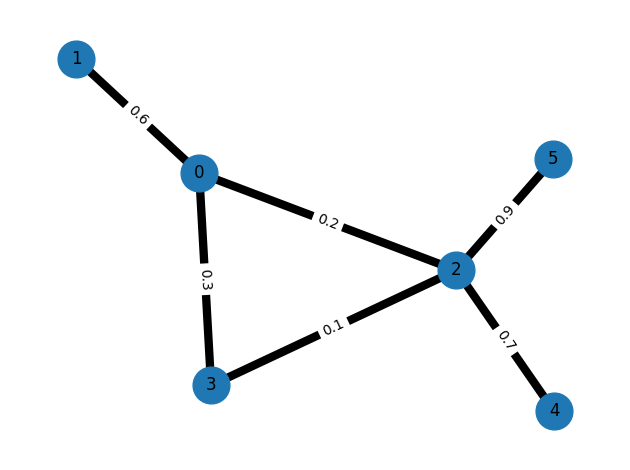
\includegraphics[width=\textwidth]{figures/toy_graph_init.png}
        \caption{Toy graph}
    \end{subfigure}
    \hfill
    \begin{subfigure}{0.3\textwidth}
        \centering
        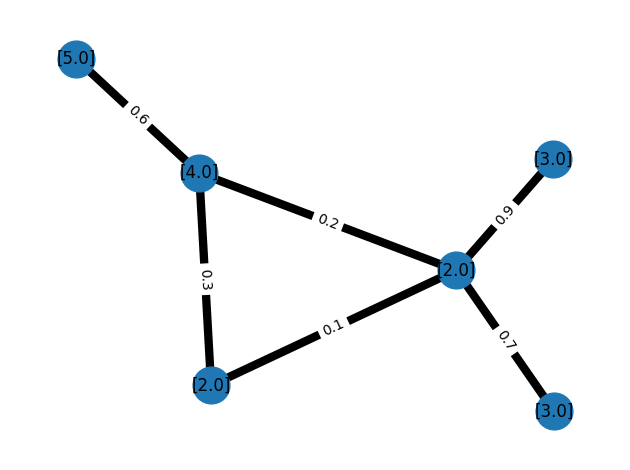
\includegraphics[width=0.45\textwidth, height=1.5cm]{figures/toy_graph_conv_K1.png}
        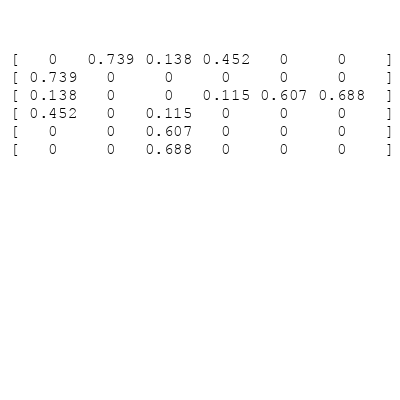
\includegraphics[width=0.45\textwidth, height=1.5cm]{figures/lap1.png}
        \caption{Convolution with $K=1$}
    \end{subfigure}
    \hfill
    \begin{subfigure}{0.3\textwidth}
        \centering
        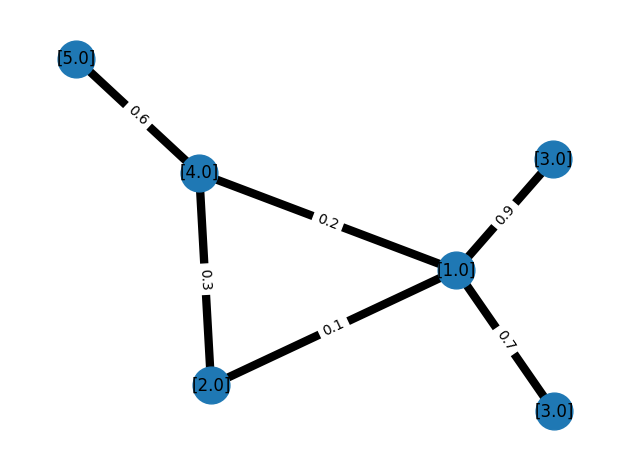
\includegraphics[width=0.45\textwidth, height=1.5cm]{figures/toy_graph_conv_K2.png}
        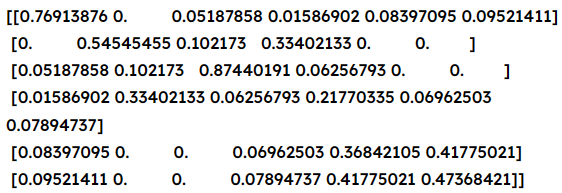
\includegraphics[width=0.45\textwidth, height=1.5cm]{figures/lap2.png}
        \caption{Convolution with $K=2$}
    \end{subfigure}
    \hfill
    \begin{subfigure}{0.3\textwidth}
        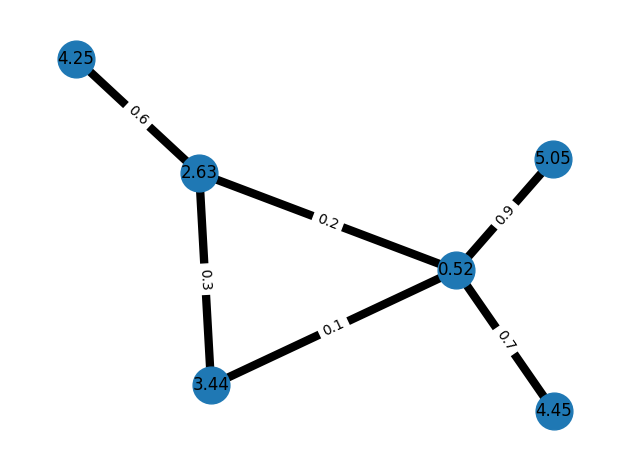
\includegraphics[width=0.45\textwidth, height=1.5cm]{figures/toy_graph_conv_K3.png}
        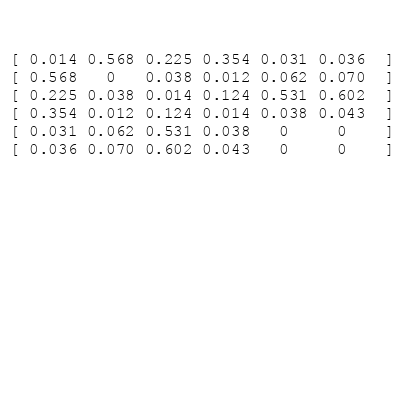
\includegraphics[width=0.45\textwidth, height=1.5cm]{figures/lap3.png}
        \caption{Convolution with $K=3$}
    \end{subfigure}
    \caption{Convolution of a toy graph and the normalized laplacian matrix $\widetilde{\mathbf{L}}^K$ for $K=1, 2, 3$.}
    \label{fig:toyGraph}
    \Description[]{illustration of convolution on graph}
 \end{figure}

\bibliographystyle{ACM-Reference-Format}
\bibliography{references}
\end{document}